\chapter{Oscillation} \label{ch:oscillation}
This chapter investigates the qualitative similarity between finite population 
short-term behavior and infinite population evolutionary limits predicted by Vose. 
It uses computation to verify predicted infinite population limits and presents 
necessary and sufficient conditions for convergence to periodic orbits. 
We compute mutation distribution $\bm{\mu}$ and crossover distribution $\bm{\chi}$ 
to satisfy those conditions. And through experiments, we explore our second research 
question that whether finite populations oscillate following infinite populations behavior.

\section{Limits}
\label{Limits}
Vose states that under mild assumptions on mutations (explained later), infinite populations converge under repeated application 
of $\mathcal{M}$ in the absense of selective pressure. Vose mentions that periodic orbits are possible, but populations converge under 
repeated application of $\mathcal{M}^2$ and the limits $\bm{p}^\ast = \lim_{n \rightarrow \infty} \mathcal{M}^{2n}({\bm p})$ 
and ${\bm q}^\ast = \lim_{n \rightarrow \infty} \mathcal{M}^{2n+1}({\bm q})$ exist (see \cite{Vose1999}).

Following Vose (see \cite{Vose1999}), let $S_g = g \mathcal{R} / \{\textbf{0}, g\}$, and let $|g|$ be the number of non zero bits in $g$. 
If $\widehat{\bm{p}}$ represents the current population in Walsh coordinates, then the next generation ${\widehat{\bm{p}}_g}^{\prime}$ 
(expressed in Walsh coordinates) is 
\[
{{\widehat{\bm{p}}}_g}^{\prime}  = \begin{cases}
    2^{\ell /2}  & \text{if $g = 0$}\\
    x_g \widehat{{\bm p}}_g + y_g(\widehat{{\bm p}}_g) & \text{otherwise}
  \end{cases}
\]
where
\[
x_g = 2\widehat{\mathcal{M}}_{g,0},  \hspace*{1cm} y_g(z) = 2^{\ell /2} \sum_{i \in S_g} z_i z_{i+g} \widehat{\mathcal{M}}_{i,i+g}.
\]

Moreover, 
\begin{eqnarray*}
|g| \;=\; 1 \nudge & \Longrightarrow & y_g = 0 \\
|g| \;>\; 0 \nudge & \Longrightarrow & |x_g| \leq 1 \\
|x_g| \;=\; 1 \nudge & \Longrightarrow & y_g = 0
\end{eqnarray*}

With above notations, the limits can be expressed in Walsh basis by recursive equations (see \cite{Vose1999})
\begin{equation}
\label{lt1}
\widehat{{\bm p}^{\ast}}_g  = \begin{cases}
    (x_g y_g(\widehat{{\bm p}^{\ast}}) + y_g(\widehat{{\bm q}^{\ast}}))/(1-x_g^2)  & \text{if $|x_g| < 0$}\\
    \widehat{p}_g  & \text{otherwise}
  \end{cases}
\end{equation}
\begin{equation}
\label{lt2}
\widehat{{\bm q}^{\ast}}_g  = \begin{cases}
    (x_g y_g(\widehat{{\bm q}^{\ast}}) + y_g(\widehat{{\bm p}^{\ast}}))/(1-x_g^2)  & \text{if $|x_g| < 0$}\\
    \widehat{\mathcal{M}({\bm p})_g}  & \text{otherwise}
  \end{cases}
\end{equation}

If $x_g \neq -1$ for all $g$, then ${\bm p}^\ast = {\bm q}^\ast = \lim_{n \rightarrow \infty} \mathcal{M}({\bm p})$ is the limit of mixing. In other cases, 
mixing converges to a periodic orbit oscillating between ${\bm p}^\ast$ and ${\bm q}^\ast = \mathcal{M}({\bm p}^\ast)$.

Limits $\widehat{{\bm p}^{\ast}}_g$ and $\widehat{{\bm q}^{\ast}_g}$ can be computed considering $g$th components in order of increasing $|g|$.
The necessary and sufficient condition for the sequence
\[
\bm{p}, \mathcal{M}({\bm p}), \mathcal{M}^2({\bm p}),\cdots
\]
to converge to a periodic orbit is that for some $g$
\begin{equation}
\label{OscCond}
-1 = \sum \limits_{j} (-1)^{g^T j} \bm{\mu}_j = - \sum \limits_{k \in \bar{g}\mathcal{R}} \bm{\chi}_{k+g} + \bm{\chi}_k
\end{equation}
 
\section{Mutation and Crossover Distributions}
The following algorithm generates mutation and crossover distributions that satisfying equation (\ref{OscCond}) 
for evolution to converge to periodic orbits. 
Let $\bm{\mu}_j$ and $\bm{\chi}_k$ represent mutation and crossover distributions respectively where $j,k \in \mathcal{R}$, 
and let $U01()$ be a random number between $0$ and $1$. For any $g \in \mathcal{R}$, $g \neq 0$, and for all $j \in \mathcal{R}$,
\[
\bm{\mu}_j = \begin{cases}
    U01() & \text{if $(g^T j)$ is odd}.\\
    0 & \text{otherwise}.
  \end{cases}
\]

Normalization of $\bm{\mu}_j$ yields $\bm{\mu}$ (the mutation distribution),
\[
\bm{\mu}_j = \bm{\mu}_j / \sum \limits_{j \in \mathcal{R} } \bm{\mu}_j.
\]
Moreover, the values $\bm{\mu}_j$ satisfy condition (\ref{OscCond}).

Condition $k \in \bar{g} \mathcal{R}$ in equation (\ref{OscCond}) is
\[
k = \bar{g} i  \text{ for some $i \in \mathcal{R}$}
\]
Multiplying through by $\bar{g}$ yields
\begin{equation*}
\bar{g} k = \bar{g} \bar{g} i \; = \; \bar{g} i \; = \; k 
\end{equation*}
The crossover distribution can therefore be generated as follows.
For all $k \in \mathcal{R}$,
\begin{eqnarray*}
\bm{\chi}_k & = & U01() \;\; if\; \bar{g}k \;=\; k \\
\bm{\chi}_{k+g} & = & U01() \;\; if\; \bar{g}k \;=\; k\\
bm{\chi}_k & = & 0  \;\; otherwise.
\end{eqnarray*} 
Normalization of $\bm{\chi}_k$ yields 
$\bm{\chi}$ (the crossover distribution),
\[
\bm{\chi}_k = \bm{\chi}_k/\sum\limits_{k \in \mathcal{R}} \bm{\chi}_k.
\]
Moreover, the values $\bm{\chi}_k$ satisfy condition (\ref{OscCond}).

\section{Initial Population}
\label{InitPopOsc}

% \begin{figure}[H]
% \begin{center}
% \resizebox*{12cm}{!}{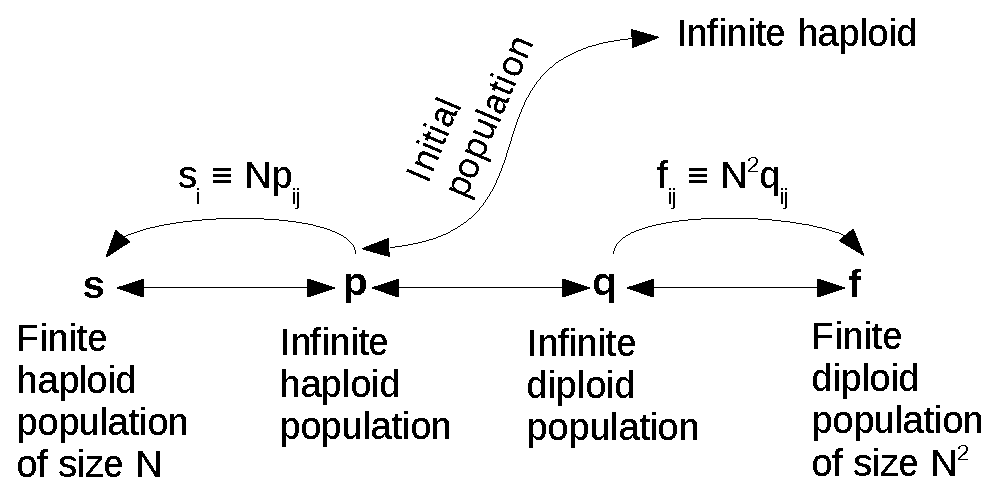
\includegraphics{figures/eps/initialpop.eps}}\hspace{4pt}
% \caption{\textbf{Initial population computation} }
% \label{initialpop}
% \end{center}
% \end{figure}
% Let finite haploid population $\bm{s}^n$, finite diploid population $\bm{f}^n$, infinite haploid population $\bm{p}^n$ 
% and infinite haploid population $\bm{q}^n$ be considered with initial population $\bm{s}^0$, $\bm{f}^0$,
% $\bm{p}^0$, $\bm{q}^0$ respectively. 
To investigate oscillating behavior of infinite population evolutionary limits 
and finite population behavior, it is desirable to have the same or corresponding initial population. 

For string length $\ell$, the number of possible haploids is $x = 2^\ell$. Let array $\bm{t}$ represent a  
population size of $N$ as follows: $\bm{t}_j$ is the $j$th population member (some element of $\{0,..,x-1\}$ 
where elements are base 2 length $\ell$ binary strings). Array $\bm{t}$ is generated from random vector $\bm{u}$ of size $x$ as follows. 
\begin{eqnarray*}
\bm{u}_i & = & U01(); \tabspace {i = 0, 1,.., x-1} \\
\bm{t}_j & = & randp(\bm{u}) ; \tabspace {j = 0,.., N-1}
\end{eqnarray*}
where $U01()$ is random number between 0 and 1, and $randp(\bm{u})$ returns random index $i$ in array $\bm{u}$ with probability $\bm{u}_i$.

Let $\bm{c}_i$ be the count of haploid member $i$ in population $\bm{t}$,
\[
\bm{c}_i = \sum \limits_{j=0}^{N-1} [\bm{t}_j = i]  \nudge; \tabspace  {i = 0,.., x-1}
\]
The infinite population vector $\bm{p}$ has $i$th component
\[
\bm{p}_i = \frac{\bm{c}_i}{ N }.
\]
This randomly generated infinite haploid population vector $\bm{p}$ is used to obtain a diploid infinite population vector $\bm{q}$,  
and finite population vectors $\bm{s}$ and $\bm{f}$ as follows.

Infinite diploid population $\bm{q}$ is calculated corresponding to initial haploid population $\bm{p}$ as
\[
\bm{q}_{i,j} = \bm{p}_i \cdot \bm{p}_j  \nudge; \tabspace  (0 \leq i,j < x).
\]

The finite haploid population members are the elements of array $\bm{t}_j$, 
the corresponding finite haploid population vector $\bm{s}$ is identical to $\bm{p}^0$. 
The finite diploid population (proportion) vector $\bm{f}$ corresponding to 
finite diploid population member array $\bm{v}$ is identical to $\bm{q}$.
% \[
% \bm{c}_i = N \cdot \bm{p}_i 
% \]
% \[
% \sum \limits_{j=0}^{N-1} [\bm{t}_j = i] = \bm{c}_i  \nudge; \tabspace  {i = 0,.., x-1} 
% \]

Thus, initial infinite haploid population vector $\bm{p}$ corresponds to initial infinite diploid 
population vector $\bm{q}$ and to initial finite 
haploid population vector $\bm{s}$ with population size $N$ and population member array $\bm{t}$ 
and to initial finite diploid population vector $\bm{f}$ with population size $N^2$ and population member array $\bm{v}$.

\section{Oscillation}
\label{Oscillation}

Crossover distribution $\bm{\chi}$ and mutation distribution $\bm{\mu}$ satisfying 
condition (\ref{OscCond}) are considered to investigate oscillating behavior between 
predicted infinite population evolutionary limits under no selective pressure.

Infinite haploid population evolutionary limits $\bm{p}_h^{\ast}$ and $\bm{q}_h^{\ast}$ 
were computed using equations (\ref{lt1}) and (\ref{lt2}). 
Infinite diploid population evolutionary limits $\bm{p}_d^{\ast}$ and $\bm{q}_d^{\ast}$ are obtained as follows
\begin{eqnarray*}
({\bm{p}_d^{\ast}})_{\langle \gamma_0, \gamma_1 \rangle} & = & ({\bm{p}_h^{\ast}})_{\gamma_0} ({\bm{p}_h^{\ast}})_{\gamma_1} \\
({\bm{q}_d^{\ast}})_{\langle \gamma_0, \gamma_1 \rangle} & = & ({\bm{q}_h^{\ast}})_{\gamma_0} ({\bm{q}_h^{\ast}})_{\gamma_1}
\end{eqnarray*}
where $\gamma = \langle \gamma_0, \gamma_1 \rangle$ is a diploid genome.

For every genome length $\ell$, the same initial population (calculated as described in (\ref{InitPopOsc})) was used for the infinite population and all 
sizes of finite populations conisdered.
Genome lengths $\ell \in \{8, \nudge10, \nudge12, \nudge14\}$ were used. Base population size of $N_0 = 64$ was used 
for the finite haploid case to compute initial population vector. The population sizes considered for plotting 
graphs were $N \in \{1N_0^2, \nudge10N_0^2, \nudge20N_0^2\}$. 
The distances of $\bm{p}^n$ and $\bm{s}^n$ to haploid evolutionary limits $\bm{p}_h^{\ast}$ and 
$\bm{q}_h^{\ast}$ were plotted and the distances of $\bm{q}^n$ and 
$\bm{f}^n$ to diploid evolutionary limits $\bm{p}_d^{\ast}$ and $\bm{q}_d^{\ast}$ were plotted. 
Distance data of finite population to infinite population were also plotted.
%oscillation


% l = 8
\begin{figure}[H]
\begin{center}
\subfloat{
\resizebox{8cm}{5cm}{\includegraphics{figures/eps/osc/b8/n004096_osc_fin_hap.eps}}} \hspace{-3em}% 
\subfloat{
\resizebox{8cm}{5cm}{\includegraphics{figures/eps/osc/b8/n004096_osc_fin_hap_dist.eps}}} \vspace{-1em}  \hspace{-3em}% 

\end{center}
\begin{center}
\subfloat{
\resizebox{8cm}{5cm}{\includegraphics{figures/eps/osc/b8/n040960_osc_fin_hap.eps}}} \hspace{-3em}% 
\subfloat{
\resizebox{8cm}{5cm}{\includegraphics{figures/eps/osc/b8/n040960_osc_fin_hap_dist.eps}}} \vspace{-1em}  \hspace{-3em}% 
\end{center}

\begin{center}
\subfloat{
\resizebox{8cm}{5cm}{\includegraphics{figures/eps/osc/b8/n081920_osc_fin_hap.eps}}} \hspace{-3em}% 
\subfloat{
\resizebox{8cm}{5cm}{\includegraphics{figures/eps/osc/b8/n081920_osc_fin_hap_dist.eps}}} \vspace{-1em}  \hspace{-3em}% 
\end{center}


\begin{center}
\subfloat{
\resizebox{8cm}{5cm}{\includegraphics{figures/eps/osc/b8/osc_inf_hap.eps}}} \hspace{-3em}%
\subfloat{
\resizebox{8cm}{5cm}{\includegraphics{figures/eps/osc/b8/fin_hap_dist.eps}}} \vspace{-0.5em} \hspace{-3em}%

\caption{\textbf{Infinite and finite haploid population oscillation behavior for genome length $\ell = 8$ (bits):} In left column, $d$ is
  distance of finite population of size $n$ or infinite population to limits for $g$ generations. In right column, $d$ is 
  distance of finite population to infinite population for $g$ generations and $d_{avg}$ is average of distance from $1$ to $50$ generations.}
\label{oscillation_8h}
\end{center}
\end{figure}


\begin{figure}[H]

\begin{center}
\subfloat{
\resizebox{8cm}{5cm}{\includegraphics{figures/eps/osc/b8/n004096_osc_fin_dip.eps}}} \hspace{-3em}% 
\subfloat{
\resizebox{8cm}{5cm}{\includegraphics{figures/eps/osc/b8/n004096_osc_fin_dip_dist.eps}}}  \vspace{-1em}  \hspace{-3em}% 
\end{center}
\begin{center}
\subfloat{
\resizebox{8cm}{5cm}{\includegraphics{figures/eps/osc/b8/n040960_osc_fin_dip.eps}}} \hspace{-3em}% 
\subfloat{
\resizebox{8cm}{5cm}{\includegraphics{figures/eps/osc/b8/n040960_osc_fin_dip_dist.eps}}}  \vspace{-1em}  \hspace{-3em}% 
\end{center}

\begin{center}
\subfloat{
\resizebox{8cm}{5cm}{\includegraphics{figures/eps/osc/b8/n081920_osc_fin_dip.eps}}} \hspace{-3em}% 
\subfloat{
\resizebox{8cm}{5cm}{\includegraphics{figures/eps/osc/b8/n081920_osc_fin_dip_dist.eps}}}  \vspace{-1em}  \hspace{-3em}% 
\end{center}

\begin{center}
\subfloat{
\resizebox{8cm}{5cm}{\includegraphics{figures/eps/osc/b8/osc_inf_dip.eps}}} \hspace{-3em}%
\subfloat{
\resizebox{8cm}{5cm}{\includegraphics{figures/eps/osc/b8/fin_dip_dist.eps}}} \vspace{-0.5em} \hspace{-3em}%

\caption{\textbf{Infinite and finite diploid population oscillation behavior for genome length $\ell = 8$ (bits):} In left column, $d$ is
  distance of finite population of size $n$ or infinite population to limits for $g$ generations. In right column, $d$ is 
  distance of finite population to infinite population for $g$ generations and $d_{avg}$ is average of distance from $1$ to $50$ generations..}
\label{oscillation_8d}
\end{center}
\end{figure}

% l = 10

\begin{figure}[H]

\begin{center}
\subfloat{
\resizebox{8cm}{5cm}{\includegraphics{figures/eps/osc/b10/n004096_osc_fin_hap.eps}}} \hspace{-3em}% 
\subfloat{
\resizebox{8cm}{5cm}{\includegraphics{figures/eps/osc/b10/n004096_osc_fin_hap_dist.eps}}} \vspace{-1em}  \hspace{-3em}% 
\end{center}
\begin{center}
\subfloat{
\resizebox{8cm}{5cm}{\includegraphics{figures/eps/osc/b10/n040960_osc_fin_hap.eps}}} \hspace{-3em}% 
\subfloat{
\resizebox{8cm}{5cm}{\includegraphics{figures/eps/osc/b10/n040960_osc_fin_hap_dist.eps}}} \vspace{-1em}  \hspace{-3em}% 
\end{center}

\begin{center}
\subfloat{
\resizebox{8cm}{5cm}{\includegraphics{figures/eps/osc/b10/n081920_osc_fin_hap.eps}}} \hspace{-3em}% 
\subfloat{
\resizebox{8cm}{5cm}{\includegraphics{figures/eps/osc/b10/n081920_osc_fin_hap_dist.eps}}} \vspace{-1em}  \hspace{-3em}% 
\end{center}

\begin{center}
\subfloat{
\resizebox{8cm}{5cm}{\includegraphics{figures/eps/osc/b10/osc_inf_hap.eps}}} \hspace{-3em}%
\subfloat{
\resizebox{8cm}{5cm}{\includegraphics{figures/eps/osc/b10/fin_hap_dist.eps}}} \vspace{-0.5em} \hspace{-3em}%

\caption{\textbf{Infinite and finite haploid population oscillation behavior for genome length $\ell = 10$ (bits):} In left column, $d$ is
  distance of finite population of size $n$ or infinite population to limits for $g$ generations. In right column, $d$ is 
  distance of finite population to infinite population for $g$ generations and $d_{avg}$ is average of distance from $1$ to $50$ generations..}
\label{oscillation_10h}
\end{center}
\end{figure}


\begin{figure}[H]

\begin{center}
\subfloat{
\resizebox{8cm}{5cm}{\includegraphics{figures/eps/osc/b10/n004096_osc_fin_dip.eps}}} \hspace{-3em}% 
\subfloat{
\resizebox{8cm}{5cm}{\includegraphics{figures/eps/osc/b10/n004096_osc_fin_dip_dist.eps}}}  \vspace{-1em}  \hspace{-3em}% 
\end{center}
\begin{center}
\subfloat{
\resizebox{8cm}{5cm}{\includegraphics{figures/eps/osc/b10/n040960_osc_fin_dip.eps}}} \hspace{-3em}% 
\subfloat{
\resizebox{8cm}{5cm}{\includegraphics{figures/eps/osc/b10/n040960_osc_fin_dip_dist.eps}}}  \vspace{-1em}  \hspace{-3em}% 
\end{center}

\begin{center}
\subfloat{
\resizebox{8cm}{5cm}{\includegraphics{figures/eps/osc/b10/n081920_osc_fin_dip.eps}}} \hspace{-3em}% 
\subfloat{
\resizebox{8cm}{5cm}{\includegraphics{figures/eps/osc/b10/n081920_osc_fin_dip_dist.eps}}}  \vspace{-1em}  \hspace{-3em}% 
\end{center}


\begin{center}
\subfloat{
\resizebox{8cm}{5cm}{\includegraphics{figures/eps/osc/b10/osc_inf_dip.eps}}} \hspace{-3em}%
\subfloat{
\resizebox{8cm}{5cm}{\includegraphics{figures/eps/osc/b10/fin_dip_dist.eps}}} \vspace{-0.5em} \hspace{-3em}%

\caption{\textbf{Infinite and finite population oscillation behavior for genome length $\ell = 10$ (bits):} In left column, $d$ is
  distance of finite population of size $n$ or infinite population to limits for $g$ generations. In right column, $d$ is 
  distance of finite population to infinite population for $g$ generations and $d_{avg}$ is average of distance from $1$ to $50$ generations..}
\label{oscillation_10d}
\end{center}
\end{figure}

% l = 12

\begin{figure}[H]

\begin{center}
\subfloat{
\resizebox{8cm}{5cm}{\includegraphics{figures/eps/osc/b12/n004096_osc_fin_hap.eps}}} \hspace{-3em}% 
\subfloat{
\resizebox{8cm}{5cm}{\includegraphics{figures/eps/osc/b12/n004096_osc_fin_hap_dist.eps}}} \vspace{-1em}  \hspace{-3em}% 
\end{center}
\begin{center}
\subfloat{
\resizebox{8cm}{5cm}{\includegraphics{figures/eps/osc/b12/n040960_osc_fin_hap.eps}}} \hspace{-3em}% 
\subfloat{
\resizebox{8cm}{5cm}{\includegraphics{figures/eps/osc/b12/n040960_osc_fin_hap_dist.eps}}} \vspace{-1em}  \hspace{-3em}% 
\end{center}
\begin{center}
\subfloat{
\resizebox{8cm}{5cm}{\includegraphics{figures/eps/osc/b12/n081920_osc_fin_hap.eps}}} \hspace{-3em}% 
\subfloat{
\resizebox{8cm}{5cm}{\includegraphics{figures/eps/osc/b12/n081920_osc_fin_hap_dist.eps}}} \vspace{-1em}  \hspace{-3em}% 
\end{center}

\begin{center}
\subfloat{
\resizebox{8cm}{5cm}{\includegraphics{figures/eps/osc/b12/osc_inf_hap.eps}}} \hspace{-3em}%
\subfloat{
\resizebox{8cm}{5cm}{\includegraphics{figures/eps/osc/b12/fin_hap_dist.eps}}} \vspace{-0.5em} \hspace{-3em}%

\caption{\textbf{Infinite and finite haploid population oscillation behavior for genome length $\ell = 12$ (bits):} In left column, $d$ is
  distance of finite population of size $n$ or infinite population to limits for $g$ generations. In right column, $d$ is 
  distance of finite population to infinite population for $g$ generations and $d_{avg}$ is average of distance from $1$ to $50$ generations..}
\label{oscillation_12h}
\end{center}
\end{figure}

\begin{figure}[H]

\begin{center}
\subfloat{
\resizebox{8cm}{5cm}{\includegraphics{figures/eps/osc/b12/n004096_osc_fin_dip.eps}}} \hspace{-3em}% 
\subfloat{
\resizebox{8cm}{5cm}{\includegraphics{figures/eps/osc/b12/n004096_osc_fin_dip_dist.eps}}}  \vspace{-1em}  \hspace{-3em}% 
\end{center}
\begin{center}
\subfloat{
\resizebox{8cm}{5cm}{\includegraphics{figures/eps/osc/b12/n040960_osc_fin_dip.eps}}} \hspace{-3em}% 
\subfloat{
\resizebox{8cm}{5cm}{\includegraphics{figures/eps/osc/b12/n040960_osc_fin_dip_dist.eps}}}  \vspace{-1em}  \hspace{-3em}% 
\end{center}

\begin{center}
\subfloat{
\resizebox{8cm}{5cm}{\includegraphics{figures/eps/osc/b12/n081920_osc_fin_dip.eps}}} \hspace{-3em}% 
\subfloat{
\resizebox{8cm}{5cm}{\includegraphics{figures/eps/osc/b12/n081920_osc_fin_dip_dist.eps}}}  \vspace{-1em}  \hspace{-3em}% 
\end{center}

\begin{center}
\subfloat{
\resizebox{8cm}{5cm}{\includegraphics{figures/eps/osc/b12/osc_inf_dip.eps}}} \hspace{-3em}%
\subfloat{
\resizebox{8cm}{5cm}{\includegraphics{figures/eps/osc/b10/fin_hap_dist.eps}}} \vspace{-0.5em} \hspace{-3em}%

\caption{\textbf{Infinite and finite diploid population oscillation behavior for genome length $\ell = 12$ (bits):} In left column, $d$ is
  distance of finite population of size $n$ or infinite population to limits for $g$ generations. In right column, $d$ is 
  distance of finite population to infinite population for $g$ generations and $d_{avg}$ is average of distance from $1$ to $50$ generations..}
\label{oscillation_12d}
\end{center}
\end{figure}


% l= 14


\begin{figure}[H]

\begin{center}
\subfloat{
\resizebox{8cm}{5cm}{\includegraphics{figures/eps/osc/b14/n004096_osc_fin_hap.eps}}} \hspace{-3em}% 
\subfloat{
\resizebox{8cm}{5cm}{\includegraphics{figures/eps/osc/b14/n004096_osc_fin_hap_dist.eps}}} \vspace{-1em}  \hspace{-3em}% 
\end{center}
\begin{center}
\subfloat{
\resizebox{8cm}{5cm}{\includegraphics{figures/eps/osc/b14/n040960_osc_fin_hap.eps}}} \hspace{-3em}% 
\subfloat{
\resizebox{8cm}{5cm}{\includegraphics{figures/eps/osc/b14/n040960_osc_fin_hap_dist.eps}}} \vspace{-1em}  \hspace{-3em}% 
\end{center}

\begin{center}
\subfloat{
\resizebox{8cm}{5cm}{\includegraphics{figures/eps/osc/b14/n081920_osc_fin_hap.eps}}} \hspace{-3em}% 
\subfloat{
\resizebox{8cm}{5cm}{\includegraphics{figures/eps/osc/b14/n081920_osc_fin_hap_dist.eps}}} \vspace{-1em}  \hspace{-3em}% 
\end{center}

\begin{center}
\subfloat{
\resizebox{8cm}{5cm}{\includegraphics{figures/eps/osc/b14/osc_inf_hap.eps}}} \hspace{-3em}%
\subfloat{
\resizebox{8cm}{5cm}{\includegraphics{figures/eps/osc/b14/fin_hap_dist.eps}}} \vspace{-0.5em} \hspace{-3em}%

\caption{\textbf{Infinite and finite haploid population oscillation behavior for genome length $\ell = 14$ (bits):} In left column, $d$ is
  distance of finite population of size $n$ or infinite population to limits for $g$ generations. In right column, $d$ is 
  distance of finite population to infinite population for $g$ generations and $d_{avg}$ is average of distance from $1$ to $50$ generations..}
\label{oscillation_14h}
\end{center}
\end{figure}

\begin{figure}[H]

\begin{center}
\subfloat{
\resizebox{8cm}{5cm}{\includegraphics{figures/eps/osc/b14/n004096_osc_fin_dip.eps}}} \hspace{-3em}% 
\subfloat{
\resizebox{8cm}{5cm}{\includegraphics{figures/eps/osc/b14/n004096_osc_fin_dip_dist.eps}}}  \vspace{-1em}  \hspace{-3em}% 
\end{center}
\begin{center}
\subfloat{
\resizebox{8cm}{5cm}{\includegraphics{figures/eps/osc/b14/n040960_osc_fin_dip.eps}}} \hspace{-3em}% 
\subfloat{
\resizebox{8cm}{5cm}{\includegraphics{figures/eps/osc/b14/n040960_osc_fin_dip_dist.eps}}}  \vspace{-1em}  \hspace{-3em}% 
\end{center}

\begin{center}
\subfloat{
\resizebox{8cm}{5cm}{\includegraphics{figures/eps/osc/b14/n081920_osc_fin_dip.eps}}} \hspace{-3em}% 
\subfloat{
\resizebox{8cm}{5cm}{\includegraphics{figures/eps/osc/b14/n081920_osc_fin_dip_dist.eps}}}  \vspace{-1em}  \hspace{-3em}% 
\end{center}

\begin{center}
\subfloat{
\resizebox{8cm}{5cm}{\includegraphics{figures/eps/osc/b14/osc_inf_dip.eps}}} \hspace{-3em}%
\subfloat{
\resizebox{8cm}{5cm}{\includegraphics{figures/eps/osc/b14/fin_dip_dist.eps}}} \vspace{-0.5em} \hspace{-3em}%

\caption{\textbf{Infinite and finite diploid population oscillation behavior for genome length $\ell = 14$ (bits):} In left column, $d$ is
  distance of finite population of size $n$ or infinite population to limits for $g$ generations. In right column, $d$ is 
  distance of finite population to infinite population for $g$ generations and $d_{avg}$ is average of distance from $1$ to $50$ generations..}
\label{oscillation_14d}
\end{center}
\end{figure}
%oscillation

\textbf{ Figures} \ref{oscillation_8h}, \ref{oscillation_8d}, \ref{oscillation_10h}, \ref{oscillation_10d}, \ref{oscillation_12h}, \ref{oscillation_12d}, 
\ref{oscillation_14h} and \ref{oscillation_14d} arranged by genome length $\ell$ in ascending order. For each genome length, figures are split into two 
cases, haploid and diploid cases of population. In each figure for unique genome length $\ell$ and population case (either haploid or diploid), sub-figures 
are arranged by population size ($N$). In each figure, first three rows of sub-figures on left column shows distance of finite population 
to limits and sub-figure in fourth row on left column shows distance of infinite population to limits. These sub-figures depicts 
oscillating behavior of both infinite and finite population when necessary and sufficient condition \ref{OscCond} is met. 
Finite population oscillation in both the haploid and diploid case is sharper with increased population size. 
As population size increases, oscillation approaches the behavior exhibited by infinite population. 

In each figure (\ref{oscillation_8h}, \ref{oscillation_8d}, \ref{oscillation_10h}, \ref{oscillation_10d}, 
\ref{oscillation_12h}, \ref{oscillation_12d}, 
\ref{oscillation_14h} and \ref{oscillation_14d}), first three rows of graphs on right side shows 
distance variation (difference in distance ($d$) and average distance ($d_{avg}$))  
where $d$ is distance between finite and infinite populations and $d_{avg}$ is average value of $d$. 
In fourth row on right, a single graph for distances ($d$) of different finite population sizes 
($N = 1N_0^2, \nudge10N_0^2, \nudge20N_0^2$) to infinite population are plotted. The resulting graphs shows distance decreases 
as population size increases which is consistent with results from section \ref{convergence}. 
The distance graphs smooth as population size increases. The graphs of $d-d_{avg}$ decreases in amplitude as population size increases.

The numerator in equation \ref{convergenceRHS} is approximately $1$. 
So from \ref{convergenceRHS}, the expected single step distance between finite and infinite population, $d$, is
\[
d \approx 1/\sqrt{N}
\]
where $N$ is the population size.
This expected single step distance is shown in table \ref{tableExpectedDistance}.
\begin{table}[ht]
\caption{\textbf{Expected single step distance $d$ for population size $N$}}
\centering
\begin{tabular}{c c c c}
\hline
$N$ & 4096 & 40960 & 81920 \\
$d$ & 0.0156 & 0.0049 & 0.0035 \\
\hline
\end{tabular}
\label{tableExpectedDistance}
\end{table}
Distance data obtained from simulations are summarized in table \ref{tableDistanceOsc}. The 
last three columns tabulate average distance values between finite and infinite population 
for population sizes $N \;=\; 4096 $, $N \;=\; 40960 $ and $N \;=\; 81920 $ respectively.
\begin{table}[ht]
\caption{\textbf{Experimental distance measured for oscillation:} $N$ is population size, $\ell$ is genome length 
and average distance between finite and infinite population is tabulated in the last three columns. $\{4096, \nudge 40960, \nudge 81920\}$ }
\centering
\begin{tabularx}{0.75\textwidth}{ c *{4}{X}}
\toprule
case & $\ell$ & $N \;=\; 4096 $ & $N \;=\; 40960 $ & $N \;=\; 81920 $\\
\midrule
\multirow{4}{*}{haploid} 	& 8 & 0.0158 & 0.0051 & 0.0035 \\
 				& 10 & 0.0157 & 0.0050 & 0.0035 \\ 
 			 	& 12 & 0.0156 & 0.0049 & 0.0035 \\
 	 			& 14 & 0.0156 & 0.0049 & 0.0035 \\ 
\midrule
\multirow{4}{*}{diploid} 	& 8 & 0.0156 & 0.0049 & 0.0035 \\
				& 10 & 0.0156 & 0.0049 & 0.0035 \\
			 	& 12 & 0.0156 & 0.0049 & 0.0035 \\
	 			& 14 & 0.0156 & 0.0049 & 0.0035 \\
\bottomrule

\end{tabularx}
\label{tableDistanceOsc}
\end{table}
Results from table \ref{tableDistanceOsc} show average distance between finite and infinite population follows closely 
the expected single step distance given in table \ref{tableExpectedDistance}. The distance decreases as $1/\sqrt{N}$.

\section{Summary}
In this chapter, we described limits predicted by Vose for infinite population, and necessary and sufficient condition 
for convergence to periodic orbits. Through experiment, we showed finite population also oscillate, 
and converge to infinite population behavior as population size increases. 
Then we studied through simulations the effect on infinite and finite population behavior of violating the condition 
for convergence to periodic orbits. Infinite population ceases to oscillate when the condition for convergence to 
periodic orbits is violated, but finite population continued to approximately oscillate for small values of $\bm{\epsilon}$. 
For smaller values of $\bm{\epsilon}$, finite population does not get aware of violation because the probability of using 
new masks created in the mutation distribution $\bm{\mu}$ and the crossover distribution $\bm{\mu}$ due to violation is very low, and 
finite population follows behavior of infinite population without violation in the condition for convergence to 
periodic orbits.





 
